\documentclass[letterpaper,10pt]{article}

\usepackage{enumitem}
\usepackage{titling}
\usepackage{listings,listings-rust}
\usepackage{url}
\usepackage{soul}
\usepackage{hyperref}
\usepackage{setspace}
\usepackage{subfig}
\usepackage{sectsty}
\usepackage{pdfpages}
\usepackage{colortbl}
\usepackage{multirow}
\usepackage{multicol}
\usepackage{relsize}
\usepackage{amsmath}
\usepackage{wasysym}
\usepackage{fancyvrb}
\usepackage[yyyymmdd]{datetime}
\usepackage{amsmath,amssymb,amsthm,graphicx,xspace}
\usepackage[titlenotnumbered,noend,noline]{algorithm2e}
\usepackage[compact]{titlesec}
\usepackage{XCharter}
\usepackage[T1]{fontenc}
\usepackage[scaled]{beramono}
\usepackage[normalem]{ulem}
\usepackage{booktabs}
\usepackage{tikz}
\usetikzlibrary{arrows.meta,automata,shapes,trees,matrix,chains,scopes,positioning,calc,decorations.pathreplacing}
\tikzstyle{block} = [rectangle, draw, fill=blue!20, 
    text width=2.5em, text centered, rounded corners, minimum height=2em]
\tikzstyle{bw} = [rectangle, draw, fill=blue!20, 
    text width=4em, text centered, rounded corners, minimum height=2em]

\definecolor{namerow}{cmyk}{.40,.40,.40,.40}
\definecolor{namecol}{cmyk}{.40,.40,.40,.40}
\renewcommand{\dateseparator}{-}

\let\LaTeXtitle\title
\renewcommand{\title}[1]{\LaTeXtitle{\textsf{#1}}}

\lstset{basicstyle=\footnotesize\ttfamily,breaklines=true}

\newcommand{\CPP}{C\nolinebreak\hspace{-.05em}\raisebox{.4ex}{\tiny\bf +}\nolinebreak\hspace{-.10em}\raisebox{.4ex}{\tiny\bf +}}
\def\CPP{{C\nolinebreak[4]\hspace{-.05em}\raisebox{.4ex}{\tiny\bf ++}}}

\newcommand{\handout}[5]{
  \noindent
  \begin{center}
  \framebox{
    \vbox{
      \hbox to 5.78in { {\bf ECE459: Programming for Performance } \hfill #2 }
      \vspace{4mm}
      \hbox to 5.78in { {\Large \hfill #4  \hfill} }
      \vspace{2mm}
      \hbox to 5.78in { {\em #3 \hfill \today} }
    }
  }
  \end{center}
  \vspace*{4mm}
}

\newcommand{\lecture}[3]{\handout{#1}{#2}{#3}{Lecture#1}}
\newcommand{\tuple}[1]{\ensuremath{\left\langle #1 \right\rangle}\xspace}

\addtolength{\oddsidemargin}{-1.000in}
\addtolength{\evensidemargin}{-0.500in}
\addtolength{\textwidth}{2.0in}
\addtolength{\topmargin}{-1.000in}
\addtolength{\textheight}{1.75in}
\addtolength{\parskip}{\baselineskip}
\setlength{\parindent}{0in}
\renewcommand{\baselinestretch}{1.5}
\newcommand{\term}{Winter 2020}

\singlespace


\begin{document}

\lecture{27 --- Liar, Liar}{\term}{Patrick Lam \& Jeff Zarnett}

I was thinking today about how humans are quite adept at building and
using tools (though not
unique\footnote{https://www.rnz.co.nz/news/national/366747/clever-kea-using-tools-to-raid-traps}). Profilers
are useful tools, but they can mislead you.  If you understand how
profilers work, you can avoid being misled.

As we've been saying this week, there are sampling-based and instrumentation-based profilers.
The tl;dr is that a sampling-based profiler can miss things, while an instrumentation-based
profiler distorts the system under observation.

Visually, sampling-based profiling can do this:
\begin{center}
	\url{https://www.youtube.com/watch?v=jQDjJRYmeWg}
\end{center}

The video's not fake; it's a real helicopter and it's really flying. What's happening, however, is that the camera is taking images at some multiple of the frequency of the blade rotation speed so it gives the illusion that the blades are not spinning at all. This is a sampling problem, and you see the same problem in car commercials on TV where it looks like the wheels are spinning backwards. They're not, but the sampling effect of the camera can make it look that way.

The main assumptions underlying sampling are that samples are ``random'' and that the sample distribution approximates the actual time-spent distribution\footnote{Lifted from ``Profilers are Lying Hobbitses'', \url{https://www.infoq.com/presentations/profilers-hotspots-bottlenecks/}, which talks about profiling for JVMs.}.

\section*{Lies from Metrics}
While app-specific metrics can lie too, mostly we'll talk about CPU
perf counters today.
In particular, we're going to look at two types of sampling-based lies.

The reference for the first type of lie is a blog post by Paul Khuong~\cite{metrics}.

This goes back to {\tt mfence}, which we've seen before. It is used, for instance, in
spinlock implementations. Khuong found that his profiles said that spinlocking didn't take much time.
But empirically: eliminating spinlocks = better than expected! Hmm.

The next step is (as we do in this course) to create microbenchmarks to better understand what's
going on. The microbenchmark contained memory accesses to uncached locations, or computations,
surrounded by store pairs/mfence/locks. He used perf to evaluate the impact of mfence vs lock.
You'll recall that perf is sampling-based and records how often the CPU is found executing each
instruction.

{\scriptsize
\begin{lstlisting}
# for locks:
$ perf annotate -s cache_misses
[...]
    0.06 :        4006b0:       and    %rdx,%r10
    0.00 :        4006b3:       add    $0x1,%r9
    ;; random (out of last level cache) read
    0.00 :        4006b7:       mov    (%rsi,%r10,8),%rbp
   30.37 :        4006bb:       mov    %rcx,%r10
    ;; foo is cached, to simulate our internal lock
    0.12 :        4006be:       mov    %r9,0x200fbb(%rip)
    0.00 :        4006c5:       shl    $0x17,%r10
    [... Skipping arithmetic with < 1% weight in the profile]
    ;; locked increment of an in-cache "lock" byte
    1.00 :        4006e7:       lock incb 0x200d92(%rip)
   21.57 :        4006ee:       add    $0x1,%rax
    [...]
    ;; random out of cache read
    0.00 :        400704:       xor    (%rsi,%r10,8),%rbp
   21.99 :        400708:       xor    %r9,%r8
    [...]
    ;; locked in-cache decrement
    0.00 :        400729:       lock decb 0x200d50(%rip)
   18.61 :        400730:       add    $0x1,%rax
    [...]
    0.92 :        400755:       jne    4006b0 <cache_misses+0x30>
\end{lstlisting}
}

We can see that in the lock situation, reads take 30 + 22 = 52\% of runtime,
while locks take 19 + 21 = 40\% of runtime.

{\scriptsize
\begin{lstlisting}
# for mfence:
$ perf annotate -s cache_misses
[...]
    0.00 :        4006b0:       and    %rdx,%r10
    0.00 :        4006b3:       add    $0x1,%r9
    ;; random read
    0.00 :        4006b7:       mov    (%rsi,%r10,8),%rbp
   42.04 :        4006bb:       mov    %rcx,%r10
    ;; store to cached memory (lock word)
    0.00 :        4006be:       mov    %r9,0x200fbb(%rip)
    [...]
    0.20 :        4006e7:       mfence 
    5.26 :        4006ea:       add    $0x1,%rax
    [...]
    ;; random read
    0.19 :        400700:       xor    (%rsi,%r10,8),%rbp
   43.13 :        400704:       xor    %r9,%r8
    [...]
    0.00 :        400725:       mfence 
    4.96 :        400728:       add    $0x1,%rax
    0.92 :        40072c:       add    $0x1,%rax
    [...]
    0.36 :        40074d:       jne    4006b0 <cache_misses+0x30>
\end{lstlisting}
}
Looks like the reads take 85\% of runtime,
while the mfence takes 15\% of runtime.

Metrics lie, though, and when you focus on the metrics as opposed to what you
actually care about, it's easy to be led astray.

In this case, what we actually care about is the total \# of cycles.

    \begin{tabular}{lr}
    No atomic/fence:& 2.81e9 cycles\\
    lock inc/dec: & 3.66e9 cycles\\
    mfence: & 19.60e9 cycles
    \end{tabular}

That 15\% number is a total lie.
Profilers, even using CPU expense counts, drastically underestimate the impact of mfence,
and overestimate the impact of locks.

This is because mfence causes a pipeline flush, and the resulting 
costs get attributed to instructions being flushed, not to the mfence itself. In other
words, mfence makes other instructions run more slowly, which camouflages its own effect
on the overall performance.


\section*{The Long Tail}

The other type of lie that sampling can hide is the one where infrequent long tails are hidden in averages.
Our source here is the blog post by Dan Luu~\cite{perf-tracing}. Suppose we have a task that's going to get distributed over multiple computers (like a search). If we look at the latency distribution, the problem is mostly that we see a long tail of events and when we are doing a computation or search where we need all the results, we can only go as the slowest step. Let's take a look at a histogram of disk read latencies, where we are performing a 64 kB read, also from that source:

\begin{center}
	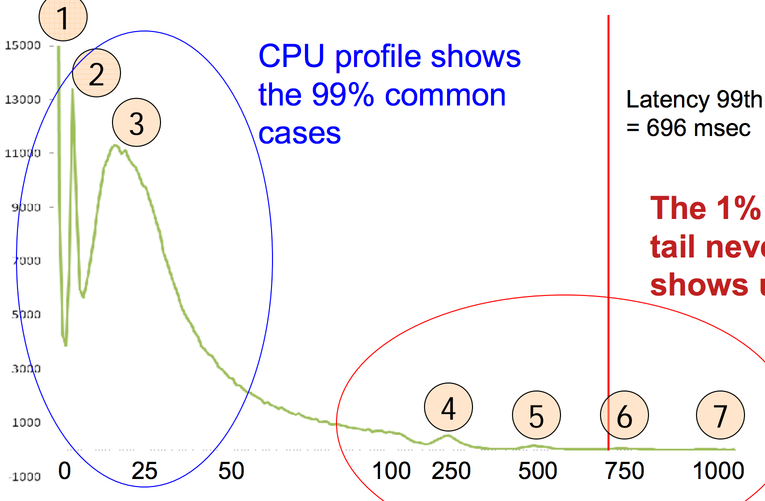
\includegraphics[width=0.5\textwidth]{images/disk_tail.png}
\end{center}

Let's break it down. Peak 1 corresponds to something cached in RAM---best case scenario. Peak 2 is at around 3ms, which is too fast for spinning and seeking magnetic hard disks, but it's fast enough for reading something from the disk cache via the PCI-Express interface. Peak 3 is obviously disk seek and read times, around 25ms. 

These numbers don't look terrible, except for the fact that we have peaks at 250, 500, 750, and 1000 ms and the 99th percentile is some 696ms which is a very, very long time. Sampling profilers are not very good at finding these things, because they throw everything into various buckets and therefore we get averages. The averages are misleading, though, because we have these weird outliers that take dramatically longer. Averages are nice as long as our data is also reasonably ``nice''.

So what actually happened? Well, from~\cite{perf-tracing}: The investigator found out that the cause was kernel throttling of the CPU for processes that went beyond their usage quota. To enforce the quota, the kernel puts all of the relevant threads to sleep until the next multiple of a quarter second. When the quarter-second hand of the clock rolls around, it wakes up all the threads, and if those threads are still using too much CPU, the threads get put back to sleep for another quarter second. The phase change out of this mode happens when, by happenstance, there aren't too many requests in a quarter second interval and the kernel stops throttling the threads. After finding the cause, an engineer found that this was happening on 25\% of disk servers at Google, for an average of half an hour a day, with periods of high latency as long as 23 hours. This had been happening for three years.

Further limitations of sampling profilers emerge, as demonstrated in this graph, also from~\cite{perf-tracing}, showing the data we get out of our sampling profiler if we take a look at Lucene (a search indexer):

\begin{center}
	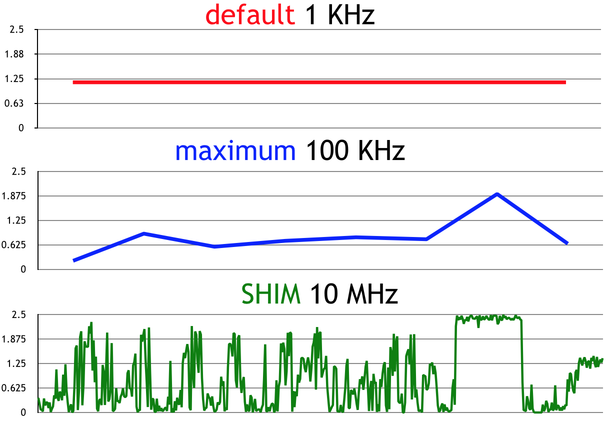
\includegraphics[width=0.3\textwidth]{images/perf-sample.png}
\end{center}

So at the default sampling interval for perf we see\ldots nothing interesting whatsoever. If we bump up to the max sampling frequency of perf, we get a moderately more interesting graph, but not much. If we use a different tool and can sample at a dramatically higher rate, then we end up with something way more useful. So we're left to wonder why does perf sample so infrequently, and how does SHIM get around this?

Well, for one thing, perf samples are done with interrupts. Processing interrupts takes a fair amount of time and if you crank up the rate of interrupts, before long, you are spending all your time handling the interrupts rather than doing useful work. So sampling tools usually don't interrupt the program too often. SHIM gets around this by being more invasive---it instruments the program, adding some periodically executed code that puts information out whenever there is an appropriate event (e.g., function return). This produces a bunch of data which can be dealt with later to produce something useful.

This instrumentation-based approach is more expensive in general, but note that DTrace\footnote{Note also the comment in the blog post: ``Yes, that includes dtrace, which I'm calling out in particular because any time you have one of these discussions, a dtrace troll will come along to say that dtrace has supported that for years. It's like the common lisp of trace tools, in terms of community trolling.''} and Nethercote's counts tool (discussed in L25) also enable custom instrumentation of select events. 

\section*{Lies from Counters}
This is fairly niche, but Rust compile hackers were trying to include
support for hardware performance counters (what perf reports) because
{\tt -Z self-profile} data was too noisy\footnote{Full story, in gory
detail,
at \url{https://hackmd.io/sH315lO2RuicY-SEt7ynGA?view}.}. Counters
are, for instance, faster than measuring time and way (i.e. 5 orders of magnitude) more deterministic.

To make counters as deterministic as possible:
\begin{itemize}[noitemsep]
\item disable Address Space Layout Randomization (randomized pointer addresses affect hash layouts);
\item subtract time spent processing interrupts (IRQs);
\item profile one thread only (if you can, in your context).
\end{itemize}
Fun fact. We talked about Spectre back in Lecture 7. Speculative execution comes up here too in terms of
counters being wrong. AMD speculates past atomics and then rolls back, but doesn't roll back perf counters.
Post-Spectre, there's a hidden model-specific register (``SpecLockMap'') that disables speculating past atomics, the kind of thing you would
want around to protect you against future things in that vein that someone might discover. Or, in better words than mine\footnote{\url{https://twitter.com/eddyb_r/status/1323587371703668742}}:

\begin{center}
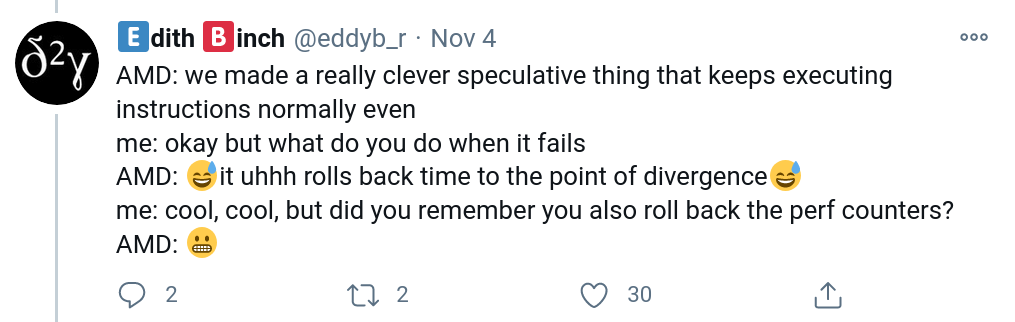
\includegraphics{images/L27-eb-tweet.png}
\end{center}

\section*{Lies about Calling Context}
This part is somewhat outdated now, as it's a pretty specific technical problem that especially arises under the {\tt gprof} tool. It's still a good example of lying tools, though,
so I'll include a condensed version. Yossi Kreinin~\cite{lies} writes about it in more detail.

gprof uses two C standard-library functions: {\bf profil()} and {\bf mcount()}.

\vspace*{-1em}
\begin{itemize}[noitemsep]
\item {\bf profil()}: asks glibc to record which instruction 
  is currently executing (100$\times$/second).
\item {\bf mcount()}: records call graph edges; called by {\tt -pg} instrumentation.
\end{itemize}
\vspace*{-1em}

Hence, {\bf profil} information is statistical, while {\bf mcount}
information is exact.  gprof can draw unreliable inferences. If you have a method \texttt{easy} and a method \texttt{hard}, each of which is called once, and \texttt{hard} takes up almost all the CPU time,
gprof might divide total time by 2 and report bogus results.

The following results from gprof are suspect (among others):
\vspace*{-1em}
\begin{itemize}[noitemsep]
  \item contribution of children to parents;
  \item total runtime spent in self+children;
\end{itemize}
\vspace*{-1em}

\paragraph{When are call graph edges right?}
Two cases:
\vspace*{-1em}
    \begin{itemize}[noitemsep]
    \item functions with only one caller
      (e.g. {\tt f()} only called by {\tt g()}); or,
    \item functions which always take the same time to complete
      (e.g. {\tt rand()}).
    \end{itemize}
\vspace*{-1em}

On the other hand, results for any function whose running time depends on its inputs,
and which is called from multiple contexts, are sketchy.


Next, we'll talk about callgrind/KCacheGrind. Like our old friends memcheck, helgrind, and cachegrind, callgrind is part of valgrind, and runs the program under an x86 JIT.  KCacheGrind is a frontend to callgrind. callgrind gives better information, but imposes
more overhead.
KCacheGrind works properly on the earlier running example, but we can still deceive it with more complicated examples.

%% \paragraph{Summary.} We've seen that some profiler results are exact;
%% some results are sampled; and some results are interpolated. If you understand the tool, you understand where it can go
%% wrong. 

%% Understand your tools!


\paragraph{Overall summary.} We saw a bunch of lies today: calling-context lies and perf attribution
lies. To avoid being bitten by lies, remember to focus on the metric you actually care about,
and understand how your tools work.



\bibliographystyle{alphaurl}
\bibliography{459}


\end{document}
